\label{sec:scheduling}
\subsection{background: scheduling}

Tor handles multiple queues of cells, for each circuit, and manages to write
cells in the outbound connection while favoring bursty over bulky traffic. The
main idea is to prioritize circuit handling interactive data streams, like chats
or web browsing. Tor uses an heuristic called EWMA~\cite{tang2010improved}
(i.e., computes the exponentially weighted moving average for the number of
cells sent on each circuit) to decide which circuit to prioritize. Recently, the
efficiency of EWMA has been improved with the Kist~\cite{jansen2014never}
scheduler used to reduce the congestion on the kernel outbound queue and push
back this delicate problem on the Tor layer.

In an ideal network, we might expect that traffic movement is an exclusive
function of the raw bandwidth capacity in each edge connection and the
scheduling algorithm implemented at each node.  The Tor network employs EWMA to
favor interactive web clients over continuous bulk clients. In moneTor, we
originally proposed to modify EWMA with a simple linear scaling factor that
would favor paid circuits.
\begin{equation}
  A_{t + \Delta t} = A_t \times 0.5^{\Delta t/H}
\end{equation}
\begin{equation}
  A'_{t + \Delta t} = A_{t + \Delta t} / \beta + C_{t, t + \Delta t}
\end{equation}
Defined in Tang and Goldeberg's original paper, $A$ is a variable score used to
sort circuits such that the circuit with the lowest $A$ is always next on the
scheduling queue. $C$ is the number of cells relayed within $\Delta t$, the time
since the previous observation, and $H$ is a global representing the half-life
decay interval in the score. Our added term, $\beta \in [1, \inf)$, is a tunable
parameter such that $Bandwidth_{premium} = Bandwidth_{nonpremium} \times \beta$
for any given circuit under ideal conditions.

\subsection{Obstacles}

Implementation into the concrete Tor infrastructure has proven to be a
considerably more complex problem. Upon failing to achieve meaningful
differentiation with low values of $\beta$, we adopted a more blunt policy which
\emph{always} services premium circuits first and implemented it in a
zero-overhead version of moneTor.\footnote{This ideal version of moneTor strips
  away all payment operations and instead passes a single signal through the
  network to distinguish premium circuits.} The results are displayed in
Figure~\ref{fig:scheduling_priority}.

\begin{figure} \centering
  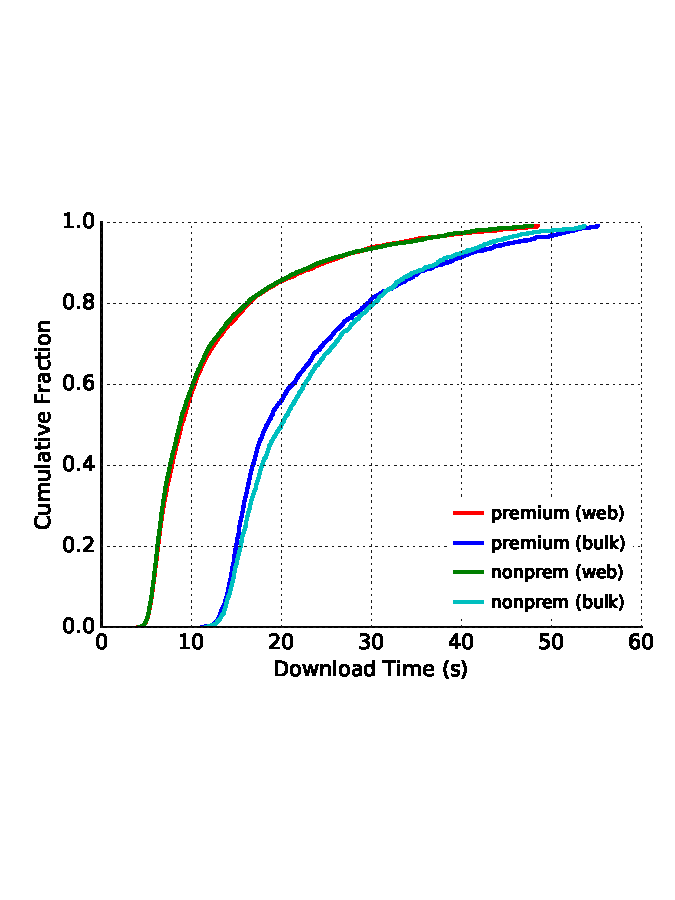
\includegraphics[trim={0 3cm 0 3cm}, clip, width=0.32\textwidth]{images/scheduling_priority.pdf}
  \caption[Prioritized Scheduling]{\textbf{Prioritized Scheduling} CDF download
    times for superimposed web and bulk clients where premium status is enforced
    only via scheduling.}
  \label{fig:scheduling_priority}
\end{figure}

Although we observed some moderate differentiation, the difference falls well
short of the benefit needed to incentivize paid users as well as our
expectations for such an inequitable scheduling policy. This result holds even
under very heavy levels of induced congestion.

\subsection{Investigation}

Our negative results can be explained if scheduling is not the most decisive
determining factor in performance. To verify this hypothesis, we studied the
incoming queue from which the scheduler is able to select new active
circuits. Figure~\ref{fig:scheduling_far} illustrates the temporal load in the
queue at a single exit relay over a one-minute time span. The height of the
curve represents the total number of cells waiting to be serviced at each
continuous point in time while the colors group quantities of cells that belong
to the same circuit. Figure~\ref{fig:scheduling_close} displays a subset of the
same information within a smaller time interval.\footnote{While the graph has
  the visual appearance of a bar graph, this is just a function of the striking
  data pattern. In actuality, the plot displays a stacked area graph.}


\begin{figure} \centering
  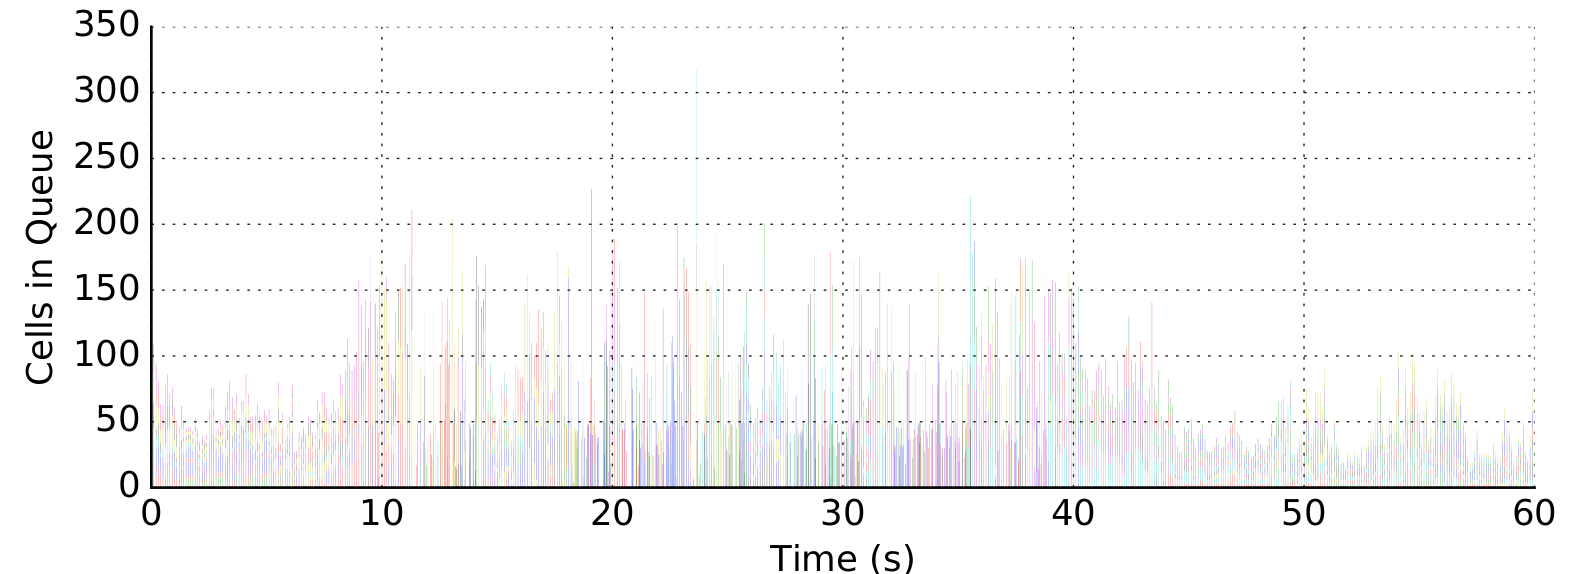
\includegraphics[width=0.5\textwidth]{images/scheduling_far.png}
  \caption[Queue Temporal Profile (60 seconds)]{\textbf{Queue Temporal Profile
      (60 seconds)} Size of the scheduling buffer over time at a single exit
    relay in terms of number of cells. Colors group cells belonging to the same circuit.}
  \label{fig:scheduling_far}
\end{figure}

\begin{figure} \centering
  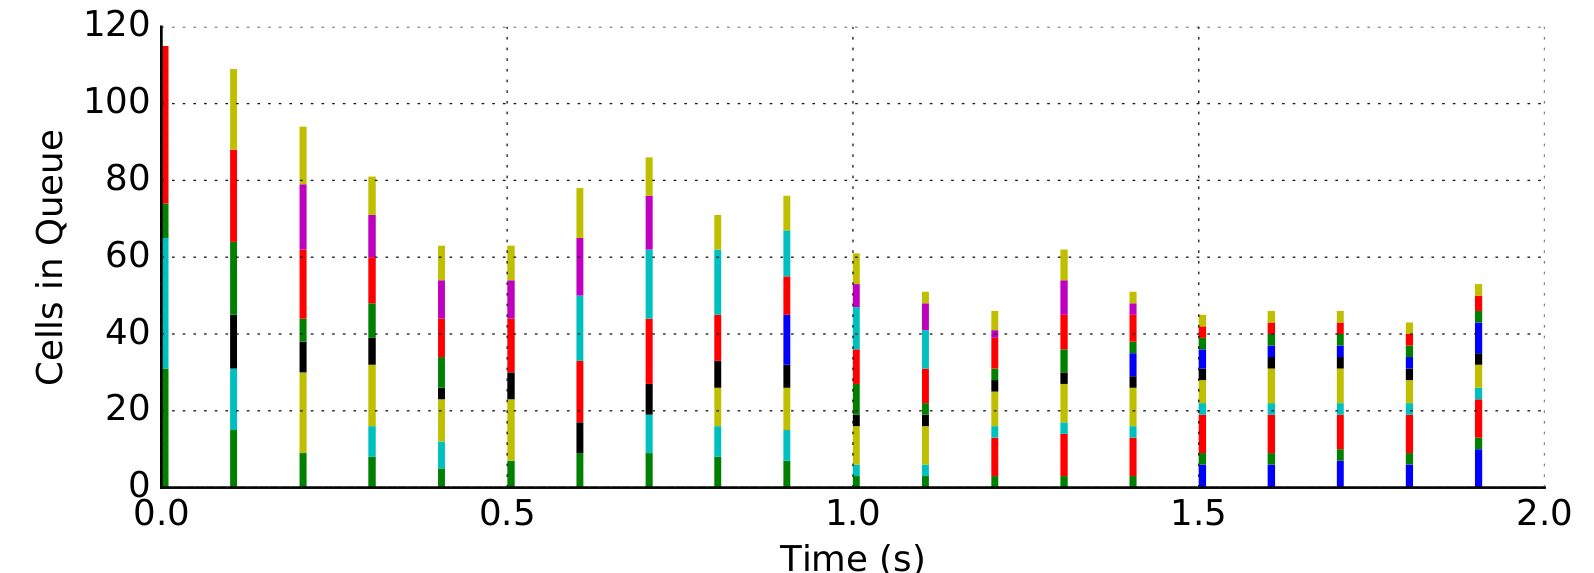
\includegraphics[width=0.5\textwidth]{images/scheduling_close.png}
  \caption[Queue Temporal Profile (2 seconds)]{\textbf{Queue Temporal Profile
      (2 seconds)} Size of the scheduling buffer over time at a single exit
    relay in terms of number of cells. Colors group cells belonging to the same
    circuit.}
  \label{fig:scheduling_close}
\end{figure}


In the aforementioned figures, notice that the queue is only populated for a
period of 10 $ms$ before it is completely flushed, implying the queue spends the
vast majority of its time empty. This 10 $ms$ window is a product of Tor's
internal event handling framework and is consistent with data from Jansen et
al~\cite{jansen2017tor}. We found in an analysis of the line-by-line
observations of the queue activity that while cells are flushed in the correct
order, they appear in the queue at roughly equal proportions. In effect,
bandwidth in our simulation is not constrained by the ordering policy of the
scheduler but rather by the rate at which they arrive from the network.

\subsection{Discussion}

There are two plausible contributing explanations. First, it may be the case
that other network control mechanisms within the Tor codebase constrain the flow
of cells, rendering the mostly idle scheduler to be ineffective. This may be
caused by any combination of point-to-point flow control, connection throttling,
or some less documented threshold embedded in the code. The positive results
covered in Section~\ref{sec:priority_exp} suggests that flow-control may play a
key role. The second explanation states that even in high-congestion, the
constraining network bottleneck does not lie within the Tor network itself but
at the exit relay interface with external servers on the web. In this scenario,
cell queuing within Tor is not nearly as important as the TCP/IP packet handling
at each exit relay.

We must emphasize that our results are in no way indicative or predictive of the
state of affairs on the live Tor network. The aforementioned experiments were
performed on a considerably smaller scale with simplistic models for network
topology and user behavior. What can be said is that networking as a whole is an
immensely complex and unpredictable domain and that the attainment of a
simulation environment conducive to effective scheduling is, at the very least,
nontrivial.
